\emph{Version \href{https://github.com/microct-ana-unibe-ch/microvasculature-manuscript/releases/tag/v1.0}{\texttt{v2.0}} of this manuscript was submitted to \href{https://www.nature.com/srep/}{Scientific Reports} and is available as a preprint at bioRχiv with the DOI \href{https://doi.org/10.1101/2023.03.08.531678}{10.1101/2023.03.08.531678}.}

The manuscript version
(\href{https://microct-ana-unibe-ch.github.io/microvasculature-manuscript/v/be7e13bbfb2a06c641670ebe5de5c4c746deea63/}{permalink})
was automatically generated
from \href{https://github.com/microct-ana-unibe-ch/microvasculature-manuscript/tree/be7e13bbfb2a06c641670ebe5de5c4c746deea63}{microct-ana-unibe-ch/microvasculature-manuscript@be7e13b}
on December 5, 2024.
Changes of this version to the submitted version are visualized \href{https://github.com/microct-ana-unibe-ch/microvasculature-manuscript/compare/v2.0.1...be7e13bbfb2a06c641670ebe5de5c4c746deea63\#files_bucket}{here on GitHub}.

\hypertarget{authors}{%
\subsection{Authors}\label{authors}}

\begin{itemize}
\item
  \textbf{David Haberthür}
  \textsuperscript{\protect\hyperlink{equal_contribution}{☯}}
  
\includegraphics[width=0.16667in,height=0.16667in]{images/orcid.svg}
  \href{https://orcid.org/0000-0003-3388-9187}{0000-0003-3388-9187}
  · 
\includegraphics[width=0.16667in,height=0.16667in]{images/github.svg}
  \href{https://github.com/habi}{habi}
  · 
\includegraphics[width=0.16667in,height=0.16667in]{images/mastodon.svg}
  \href{https://mastodon.social/@habi}{@habi@mastodon.social}
  Institute of Anatomy, University of Bern, Baltzerstrasse 2, CH-3012 Bern, Switzerland
\item
  \textbf{Oleksiy-Zakhar Khoma}
  \textsuperscript{\protect\hyperlink{equal_contribution}{☯}}
  
\includegraphics[width=0.16667in,height=0.16667in]{images/orcid.svg}
  \href{https://orcid.org/0000-0002-1914-6873}{0000-0002-1914-6873}
  · 
\includegraphics[width=0.16667in,height=0.16667in]{images/github.svg}
  \href{https://github.com/ol-khoma}{ol-khoma}
  Institute of Anatomy, University of Bern, Baltzerstrasse 2, CH-3012 Bern, Switzerland
\item
  \textbf{Tim Hoessly}
  Institute of Anatomy, University of Bern, Baltzerstrasse 2, CH-3012 Bern, Switzerland
\item
  \textbf{Eugenio Zoni}
  Department for BioMedical Research, Urology Research Laboratory, University of Bern, Bern, Switzerland; Department of Urology, Inselspital, Bern University Hospital, Bern, Switzerland
\item
  \textbf{Marianna Kruithof-de Julio}
  
\includegraphics[width=0.16667in,height=0.16667in]{images/orcid.svg}
  \href{https://orcid.org/0000-0002-6085-7706}{0000-0002-6085-7706}
  Department for BioMedical Research, Urology Research Laboratory, University of Bern, Bern, Switzerland; Department of Urology, Inselspital, Bern University Hospital, Bern, Switzerland; Department for BioMedical Research, Translation Organoid Research, University of Bern, Bern, Switzerland
\item
  \textbf{Stewart D. Ryan}
  
\includegraphics[width=0.16667in,height=0.16667in]{images/orcid.svg}
  \href{https://orcid.org/0000-0001-7016-771X}{0000-0001-7016-771X}
  U-Vet Hospital, University of Melbourne Veterinary School, Werribee, Australia
\item
  \textbf{Myriam Grunewald}
  
\includegraphics[width=0.16667in,height=0.16667in]{images/orcid.svg}
  \href{https://orcid.org/0000-0001-5394-9218}{0000-0001-5394-9218}
  Department of Developmental Biology and Cancer Research, Faculty of Medicine, The Hebrew University, Organoid Research Center, Hadassah University Hospital, Jerusalem, Israel
\item
  \textbf{Benjamin Bellón}
  
\includegraphics[width=0.16667in,height=0.16667in]{images/orcid.svg}
  \href{https://orcid.org/0000-0003-2297-9160}{0000-0003-2297-9160}
  Preclinical and Translational Research, Institut Straumann AG, Basel, Switzerland
\item
  \textbf{Rebecca Sandgren}
  
\includegraphics[width=0.16667in,height=0.16667in]{images/orcid.svg}
  \href{https://orcid.org/0000-0003-4473-4666}{0000-0003-4473-4666}
  Centre for Comparative Medicine, Medical Faculty, Lund University, Lund, Sweden
\item
  \textbf{Stephan Handschuh}
  
\includegraphics[width=0.16667in,height=0.16667in]{images/orcid.svg}
  \href{https://orcid.org/0000-0002-2140-7892}{0000-0002-2140-7892}
  VetCore Facility for Research, Imaging Unit, University of Veterinary Medicine, Vienna, Austria
\item
  \textbf{Benjamin E. Pippenger}
  
\includegraphics[width=0.16667in,height=0.16667in]{images/orcid.svg}
  \href{https://orcid.org/0000-0001-7990-5555}{0000-0001-7990-5555}
  Preclinical and Translational Research, Institut Straumann AG, Basel, Switzerland; Department of Periodontology, University of Bern, Bern, Switzerland
\item
  \textbf{Dieter Bosshardt}
  
\includegraphics[width=0.16667in,height=0.16667in]{images/orcid.svg}
  \href{https://orcid.org/0000-0002-2132-6363}{0000-0002-2132-6363}
  Department of Periodontology, University of Bern, Bern, Switzerland
\item
  \textbf{Valentin Djonov}
  
\includegraphics[width=0.16667in,height=0.16667in]{images/orcid.svg}
  \href{https://orcid.org/0000-0002-5062-1169}{0000-0002-5062-1169}
  Institute of Anatomy, University of Bern, Baltzerstrasse 2, CH-3012 Bern, Switzerland
\item
  \textbf{Ruslan Hlushchuk}
  \textsuperscript{\protect\hyperlink{correspondence}{✉}}
  
\includegraphics[width=0.16667in,height=0.16667in]{images/orcid.svg}
  \href{https://orcid.org/0000-0002-6722-8996}{0000-0002-6722-8996}
  · 
\includegraphics[width=0.16667in,height=0.16667in]{images/github.svg}
  \href{https://github.com/RuslanHlushchuk}{RuslanHlushchuk}
  Institute of Anatomy, University of Bern, Baltzerstrasse 2, CH-3012 Bern, Switzerland
\end{itemize}

\leavevmode\vadjust pre{\hypertarget{equal_contribution}{}}%
☯ --- David Haberthür and
Oleksiy-Zakhar Khoma contributed equally to this work.

\leavevmode\vadjust pre{\hypertarget{correspondence}{}}%
✉ --- Corresponding author: Ruslan Hlushchuk (\href{mailto:ruslan.hlushchuk@unibe.ch}{\nolinkurl{ruslan.hlushchuk@unibe.ch}}, \href{tel:+41\%2031\%20684\%2046\%2080}{+41 31 684 46 80}).

\hypertarget{abstract}{%
\subsection{Abstract}\label{abstract}}

Angiogenesis is essential for skeletal development, bone healing, and regeneration.
Improved non-destructive, three-dimensional (3D) imaging of the vasculature within bone tissue would benefit many research areas, especially implantology and tissue engineering.

X-ray microtomography (microCT) is a well-suited non-destructive 3D imaging technique for bone morphology.
For microCT-based detection of vessels, it is paramount to use contrast enhancement.
Limited differences in radiopacity between perfusion agents and mineralized bone make their distinct segmentation problematic and have been a major drawback of this approach.
A decalcification step resolves this issue but inhibits the simultaneous assessment of bone microstructure and vascular morphology.
The problem of contrasting becomes further compounded in samples with metal implants.

This study describes μAngiofil-enhanced microCT-based visualization of vasculature within bone tissue in small and large animal models, with and without decalcification.
We present simultaneous microvascular and bone imaging in murine tibia, a murine bone metastatic model, the pulp chamber, gingiva, and periodontal ligaments.
In a large animal model (minipig), we perform visualization and segmentation of different tissue types and vessels in the hemimandible containing metal implants.
Moreover, we show the potential of the dual-energy approach in facilitating the distinction between bone tissue and the applied contrast agent.

Our manuscript introduces the first non-destructive approach for 3D imaging of the vasculature within soft and hard tissues in the vicinity of metal implants in a large animal model.

\hypertarget{introduction}{%
\subsection{Introduction}\label{introduction}}

Angiogenesis, the formation of new blood vessels from preexisting vessels, is crucial for skeletal development as well as for bone healing and regeneration\textsuperscript{\protect\hyperlink{ref-zXoIXG3G}{1}--\protect\hyperlink{ref-Vu36g0cK}{5}}.
In addition to carrying nutrients and growth factors, those newly formed blood vessels are a delivery route of stem cells and progenitor cells to the bone-defect site\textsuperscript{\protect\hyperlink{ref-dBkW39I8}{6}--\protect\hyperlink{ref-5mgeUNd6}{8}}.
In the case of bone grafts, many synthetic ones fail to bridge critically sized defects due to their inability to promote vascularization\textsuperscript{\protect\hyperlink{ref-Vu36g0cK}{5},\protect\hyperlink{ref-33Vq8bQx}{9}}.
The structural nature of skeletal tissue makes three-dimensional (3D) imaging of its vasculature extremely difficult.
Histology, a destructive and two-dimensional approach, remains a gold standard for assessing vasculature in bones\textsuperscript{\protect\hyperlink{ref-117R9ULnv}{10}}.

Classic soft tissue imaging techniques such as light sheet microscopy or confocal laser scanning microscopy face challenges in their application due to the encasement of blood vessels in calcified tissue\textsuperscript{\protect\hyperlink{ref-117R9ULnv}{10}}.
Despite recent advances in tissue clearing-based imaging methods for craniofacial and other bones\textsuperscript{\protect\hyperlink{ref-ZGzobRpX}{11}--\protect\hyperlink{ref-X0aG1K2m}{13}} as well as for the whole body\textsuperscript{\protect\hyperlink{ref-BNZSaEBe}{14}}, the application of such methods remains challenging and is mainly limited to small animal models.
Simultaneous non-destructive 3D imaging of the vasculature within bone tissue and of the bone tissue itself, especially in the case of larger bone grafts, has been a challenge for decades\textsuperscript{\protect\hyperlink{ref-Vu36g0cK}{5},\protect\hyperlink{ref-1FUMXJVtA}{15}}.
Thus, many research areas benefit from improved three-dimensional imaging of the vasculature within bone tissue, for example, bone biology, bone metastatic disease, tissue engineering, implantology, and reconstructive surgery.

In the last decades, X-ray micro-computed tomography (microCT) gained recognition as a non-destructive 3D imaging technique for bone morphology\textsuperscript{\protect\hyperlink{ref-KjvwGWK2}{16}}.
Due to the inherently low difference in X-ray absorption levels between vessels and different soft tissues, it is not easily feasible to distinguish such structures within the bone.
To unambiguously detect vasculature within bone it is thus necessary to instill the vessels with either a contrast agent or use a casting method to otherwise fill the blood vessels.
Currently, existing protocols for imaging the vasculature within the bone via vascular replica have drawbacks, like showing disjoint vascular components or completely missing vascular segments\textsuperscript{\protect\hyperlink{ref-117R9ULnv}{10},\protect\hyperlink{ref-168Ee16HU}{17}}.
The minor contrast difference between the perfusion agent used to generate the vascular network replica and the mineralized bone makes it problematic to distinguish bone tissue and vasculature.
To enable proper visualization and segmentation of vasculature within bone tissue, decalcifying the bone samples has become practically a standard method\textsuperscript{\protect\hyperlink{ref-AHsHFIUt}{2},\protect\hyperlink{ref-117R9ULnv}{10}}.
Such a decalcification procedure makes a simultaneous assessment of bone microstructure and vascular morphology impossible\textsuperscript{\protect\hyperlink{ref-117R9ULnv}{10}}.
However in a recent study by Rosenblum et al.\textsuperscript{\protect\hyperlink{ref-yP3RkDdM}{18}}, in a small animal model study without biomedical implants, it was shown that this limitation can be overcome by iterative microCT-imaging (pre- and post-decalcification).

Intravascular contrast-agent-enhanced microCT has the potential to overcome these issues.
It has become a method of choice for the evaluation of angiogenesis in bone tissue engineering and remodeling applications\textsuperscript{\protect\hyperlink{ref-AHsHFIUt}{2},\protect\hyperlink{ref-Vu36g0cK}{5},\protect\hyperlink{ref-13YRlKdu2}{19}}.
Barium sulfate and Microfil have been applied as the two most common contrast agents in studies on the vascularization of bone tissue.
Only some selected studies\textsuperscript{\protect\hyperlink{ref-AHsHFIUt}{2}} managed to show better perfusion and thus visualization when perfusing the vasculature with barium sulfate.
Previous studies have reported disadvantages associated with barium sulfate suspensions, including higher viscosity, which can sometimes result in incomplete vascular filling and weak or inhomogeneous signal, particularly in higher resolution scans\textsuperscript{\protect\hyperlink{ref-AHsHFIUt}{2}}.
These issues may be attributed to particle aggregation, as indicated by various studies\textsuperscript{\protect\hyperlink{ref-DWiXWNoA}{20}--\protect\hyperlink{ref-Ror9Uhfa}{22}}.
Although Microfil has probably been applied in a larger number of vasculature imaging studies than barium sulfate, Microfil was reported to have disadvantages like vascular damage\textsuperscript{\protect\hyperlink{ref-1A0HsmRho}{23}} as well as poor or incomplete filling of the vasculature\textsuperscript{\protect\hyperlink{ref-AHsHFIUt}{2},\protect\hyperlink{ref-KJUjdwi7}{21},\protect\hyperlink{ref-Ror9Uhfa}{22}}.

In the study of tumor models\textsuperscript{\protect\hyperlink{ref-cNoYNu8B}{24}}, assessing and non-destructively imaging tumor vasculature in 3D is a demanding task.
Due to the intraosseous location, imaging is even more challenging in a bone metastatic disease model.
Changes in bone and vasculature are of crucial importance for the progression of bone metastatic disease.
Therefore, simultaneous imaging of bone and vasculature is highly desired, making a decalcification step unfavorable.
It is thus of paramount importance to develop an imaging method for the assessment of tumor vasculature in the bone without decalcification, which renders bone microstructure X-ray transparent.
In this manuscript, we present such a method for visualizing intratumoral vasculature and defects in mineralized bone tissue.

The craniofacial skeleton, including the mandible, is a frequent location for distraction osteogenesis as well as other forms of bone regeneration and repair, for which vascularization is important\textsuperscript{\protect\hyperlink{ref-yZTJBX1B}{4},\protect\hyperlink{ref-18wESlA6d}{25}}.
Even though metal implants have revolutionized the treatment of patients with missing teeth or injured joints and bones\textsuperscript{\protect\hyperlink{ref-11349lK8v}{26},\protect\hyperlink{ref-rCXuqa0O}{27}}, they are problematic for tomographic image acquisition.
The problem of imaging the vasculature becomes even further compounded in their presence, for example when studying vascularization in a jaw with metal implants.
Due to their high X-ray absorption, metal implants produce beam hardening, partial volume, and low signal artifacts in the resulting tomographic datasets\textsuperscript{\protect\hyperlink{ref-X5Wzek9s}{28}}.
Interactions occurring at the tissue-implant interface are widely believed to play a crucial role in the success of implant placement and healing\textsuperscript{\protect\hyperlink{ref-11349lK8v}{26},\protect\hyperlink{ref-137VU0bph}{29}}.
High-resolution tomographic imaging of the tissue-implant interface is complicated due to artifacts from the metal implants in the resulting datasets.
Imaging with increased acceleration voltage and at small resolutions alleviates these imaging artifacts.
MicroCT imaging is the only available approach to non-destructively investigate the intact bone-implant interface in both 3D\textsuperscript{\protect\hyperlink{ref-11349lK8v}{26}} and in proximity to the implant surface (i.e.~closer than 100 μm).

Implantology and osteology studies are often conducted in large animal models rendering the corresponding imaging even more complicated due to the lack of transgenic lines as well as the larger size of the harvested samples.
The Göttingen Minipig is widely recognized as a valuable large animal model in preclinical dental and orofacial research, mainly because of its anatomical similarities to humans\textsuperscript{\protect\hyperlink{ref-Siy9vGW7}{30}--\protect\hyperlink{ref-1EXdAADA3}{32}}.
Its bone structure and bone remodeling processes closely resemble those of humans, further enhancing its suitability for such studies, including ours.

The present study introduces a technique for high-resolution microCT-based visualization of microvasculature within bone tissue in small and large animal models, both with and without decalcification of the bone.
Moreover, we show that the polymer-based contrast agent μAngiofil is suitable for simultaneous imaging and subsequent analysis of peri-implant hard and soft tissues as well as their vascularization in the vicinity of metal implants in a large animal model.

\hypertarget{materials-methods-and-results}{%
\subsection{Materials, Methods, and Results}\label{materials-methods-and-results}}

\hypertarget{animals}{%
\subsubsection{Animals}\label{animals}}

In this study, we used one 21-month-old transgenic VEGF male mouse (see\textsuperscript{\protect\hyperlink{ref-nC0ZZVgL}{33}} for more details), five CB17SCID male mice, three C57BL/6 mice, and two Göttingen minipigs.
Animal procedures were performed in accordance with the applicable Swedish, Israeli, or Swiss legislation on the protection of animals and were approved by the corresponding committees.

Murine experiments were approved by the local Swiss ethical committee (Tierversuchskommission des Kantons Bern, Amt für Veterinärwesen, Bern, Switzerland) under permit number BE 55/16.
Minipig experiments were approved by the Malmö/Lund Ethics Committee on Animal Testing at the Lund District Court, Sweden under license 5.8.18-15672/2019.

The following reporting adheres to the ARRIVE Guidelines 2.0\textsuperscript{\protect\hyperlink{ref-1ppOkyPO}{34}} for relevant items.

\hypertarget{tomographic-imaging}{%
\subsubsection{Tomographic imaging}\label{tomographic-imaging}}

For this study, we imaged all samples with different Bruker SkyScan X-ray microtomography scanners.
An overview of the relevant scanning and reconstruction parameters is given in the text below.
A table listing all the scanning and reconstruction parameters of all the performed scans is given in the \protect\hyperlink{supplementary-materials}{Supplementary Materials}.

\hypertarget{contrast-enhanced-microangioct-of-mice-using-ux3bcangiofil}{%
\paragraph{Contrast-enhanced microAngioCT of mice using μAngiofil}\label{contrast-enhanced-microangioct-of-mice-using-ux3bcangiofil}}

The contrast agent μAngiofil (Fumedica AG, Switzerland) was prepared according to the manufacturer's recommendations.
The perfusion of the mice was performed as previously described\textsuperscript{\protect\hyperlink{ref-s9aC9H1e}{35},\protect\hyperlink{ref-ijqzbOI6}{36}}.
Heparinized animals were deeply anesthetized with a mixture of fentanyl (0.05 mg/kg), midazolam (5 mg/kg), and medetomidine (0.5 mg/kg).
The thorax and the peritoneal cavity were opened with scissors to expose the descending aorta.
The exposed aorta was then cannulated in either antegrade (for the perfusion of the hind limbs) or retrograde direction (for the perfusion of the head and teeth) with a Venflon cannula (26 GA).
Afterward, the blood was flushed out with a warm PBS solution.
Several cuts of the liver edge allowed for drainage of the blood and buffer solution.
Thereafter, the selected part of the body (hind limbs or head and teeth) was perfused with μAngiofil at 1--1.5 ml/min using a syringe pump.
The perfusion lasted until the organ of interest appeared completely filled with the blue contrast agent\textsuperscript{\protect\hyperlink{ref-ijqzbOI6}{36},\protect\hyperlink{ref-TYAmre95}{37}}.
In bones, it is not possible to visually monitor this color change, thus perfusion of the neighboring soft tissues serves as an indirect marker of sufficient perfusion within the bone.
To achieve correct perfusion of the vessels within the bone, we prolonged the perfusion time by instilling at least 2 ml of extra volume of contrast agent after all the superficial tissues of the extremity or head turned blue.
After μAngiofil polymerization, samples were fixed in a 4 \% paraformaldehyde (PFA) solution at 4 °C and stored in PFA until tomographic imaging.
Samples were then imaged using a SkyScan 1172 (Version F, control software version 1.5 (build 26), Bruker microCT N.V., Kontich, Belgium).
For imaging, the samples were removed from the PFA solution, wrapped in closed-pore foam, and scanned in a custom-made sealed plastic sample holder under humid conditions.
Tomographic imaging was performed with an X-ray source acceleration voltage of 49 kV and an X-ray source current of 200 μA.
Projection images were recorded over a sample rotation of 360°, with one projection acquired at every 0.05° with 3 projections averaged for noise reduction.
Each projection image with a size of 4000 x 2672 pixels was exposed for 985 ms.
This resulted in datasets with an isotropic voxel size of 2.99 μm.

Figure \ref{fig:1} shows the bone microstructure and vascularization of a tibia of a 21-month-old VEGF transgenic male mouse.
This visualization approach enables the simultaneous display of bone and its vascularization.
These tomographic datasets were also used in another study\textsuperscript{\protect\hyperlink{ref-nC0ZZVgL}{33}}, where we performed simultaneous quantification of vasculature and bone volume.

\begin{figure}
\hypertarget{fig:1}{%
\centering
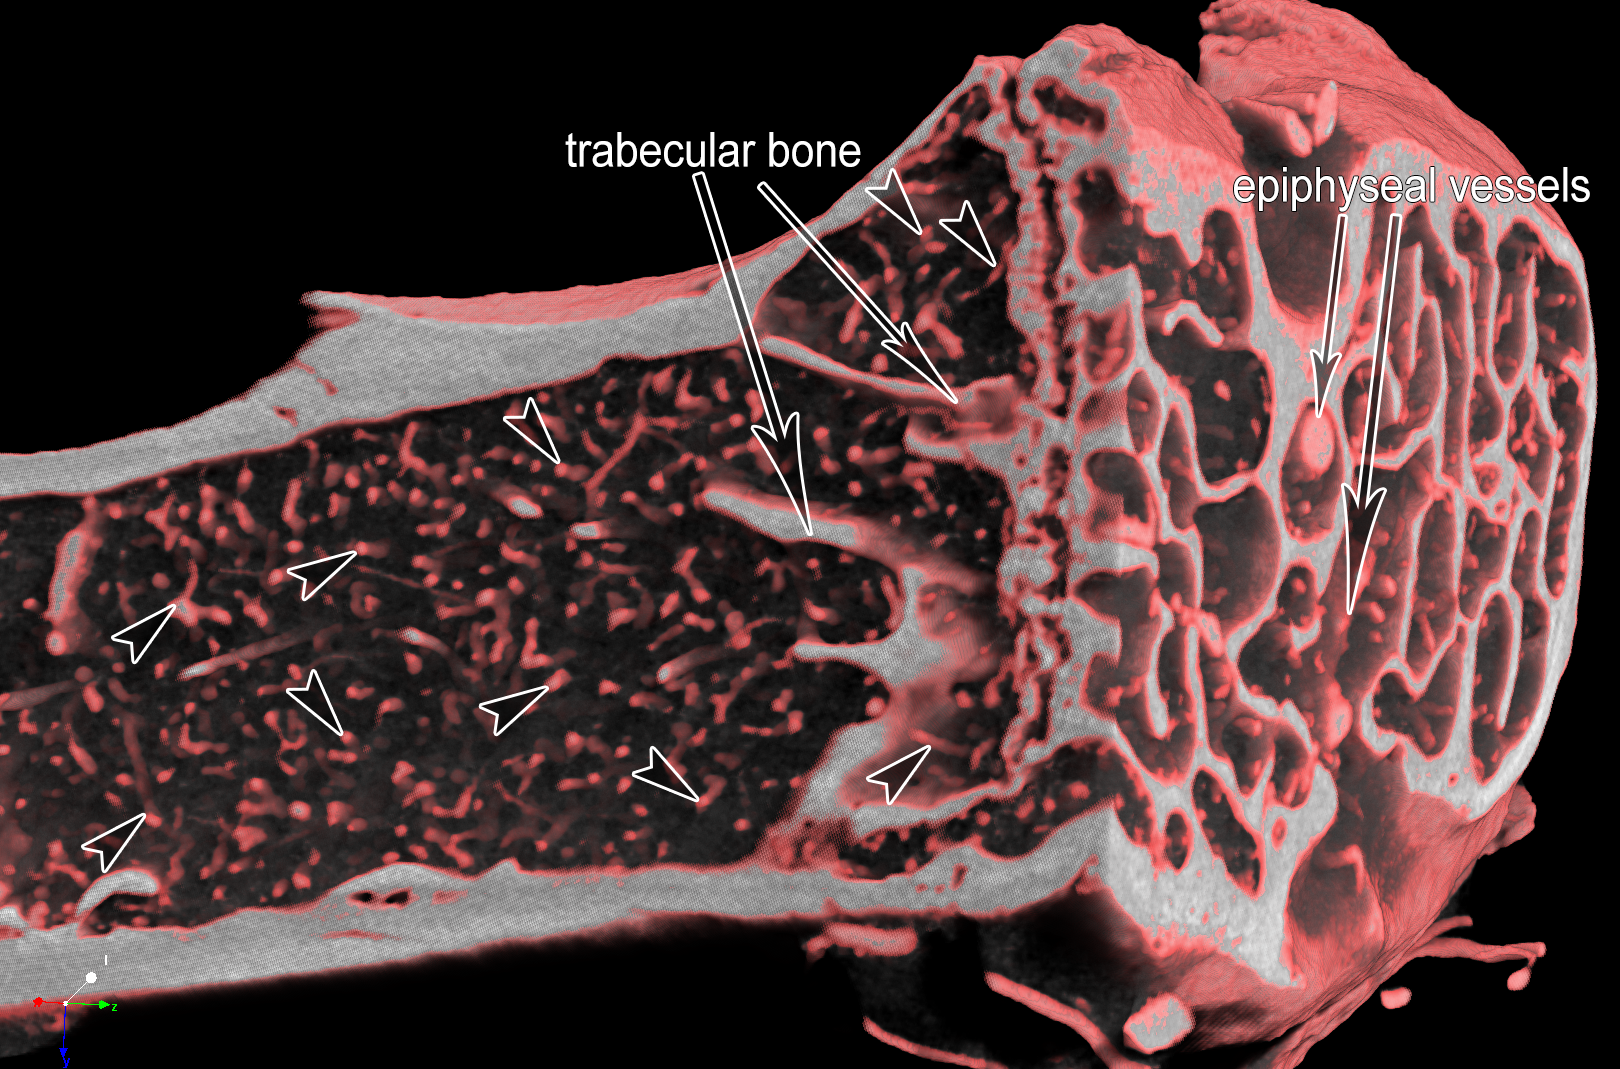
\includegraphics{images/Fig1_murine_tibia.png}
\caption{\textbf{microAngioCT of the proximal murine tibia of a 21-month-old VEGF transgenic male mouse.}
After perfusion with μAngiofil, the murine tibia was harvested, fixated in 4 \% PFA and imaged by microCT.
Arrowheads mark microvessels within the tibia.
The diameter of the tibia shaft is around 1 mm.
On the right side of the image, one can distinguish the bigger epiphyseal vessels.
The bone tissue appears white at the plane of the virtual section through the microCT-dataset.}\label{fig:1}
}
\end{figure}

\hypertarget{decalcification-of-the-ux3bcangiofil-perfused-murine-tibia}{%
\paragraph{Decalcification of the μAngiofil-perfused murine tibia}\label{decalcification-of-the-ux3bcangiofil-perfused-murine-tibia}}

We successfully established a bone decalcifying protocol (for murine hind limb) with 10\% ethylenediamine tetra-acetic acid (EDTA) solution\textsuperscript{\protect\hyperlink{ref-iM9i6gkJ}{38}} by adapting previous work\textsuperscript{\protect\hyperlink{ref-168Ee16HU}{17}}.

Decalcification of bone tissue does not negatively influence the bone structure itself, but reduces the X-ray absorption of bone tissue and thus makes it impossible to visualize it simultaneously with the vasculature (Fig. \ref{fig:2} B).

As described above, we instilled the lower body of 10-week-old CB17SCID male mice with μAngiofil.
Following polymerization of the contrast agent, the hind limbs were collected, fixed in 4 \% PFA, and stored in PFA until scanning.
After an initial tomographic scan, the hind limbs were decalcified in 10\% EDTA (pH 7.5) at room temperature for 7 days, followed by a second tomographic scan of the sample.

These samples were imaged with a SkyScan 1172 (Version F, control software version 1.5 (build 23), Bruker microCT N.V., Kontich, Belgium), with an X-ray source acceleration voltage of 59 kV and an X-ray source current of 167 μA.
The X-ray spectrum was filtered by 0.25 mm of aluminum.
Projection images were recorded over a sample rotation of 180°, with one projection acquired at every 0.1° with 2 projections averaged for noise reduction.
Each projection image with a size of 4000 x 2672 pixels was exposed for 1740 ms.
This resulted in an isotropic voxel size of 3.19 μm.

\begin{figure}
\hypertarget{fig:2}{%
\centering
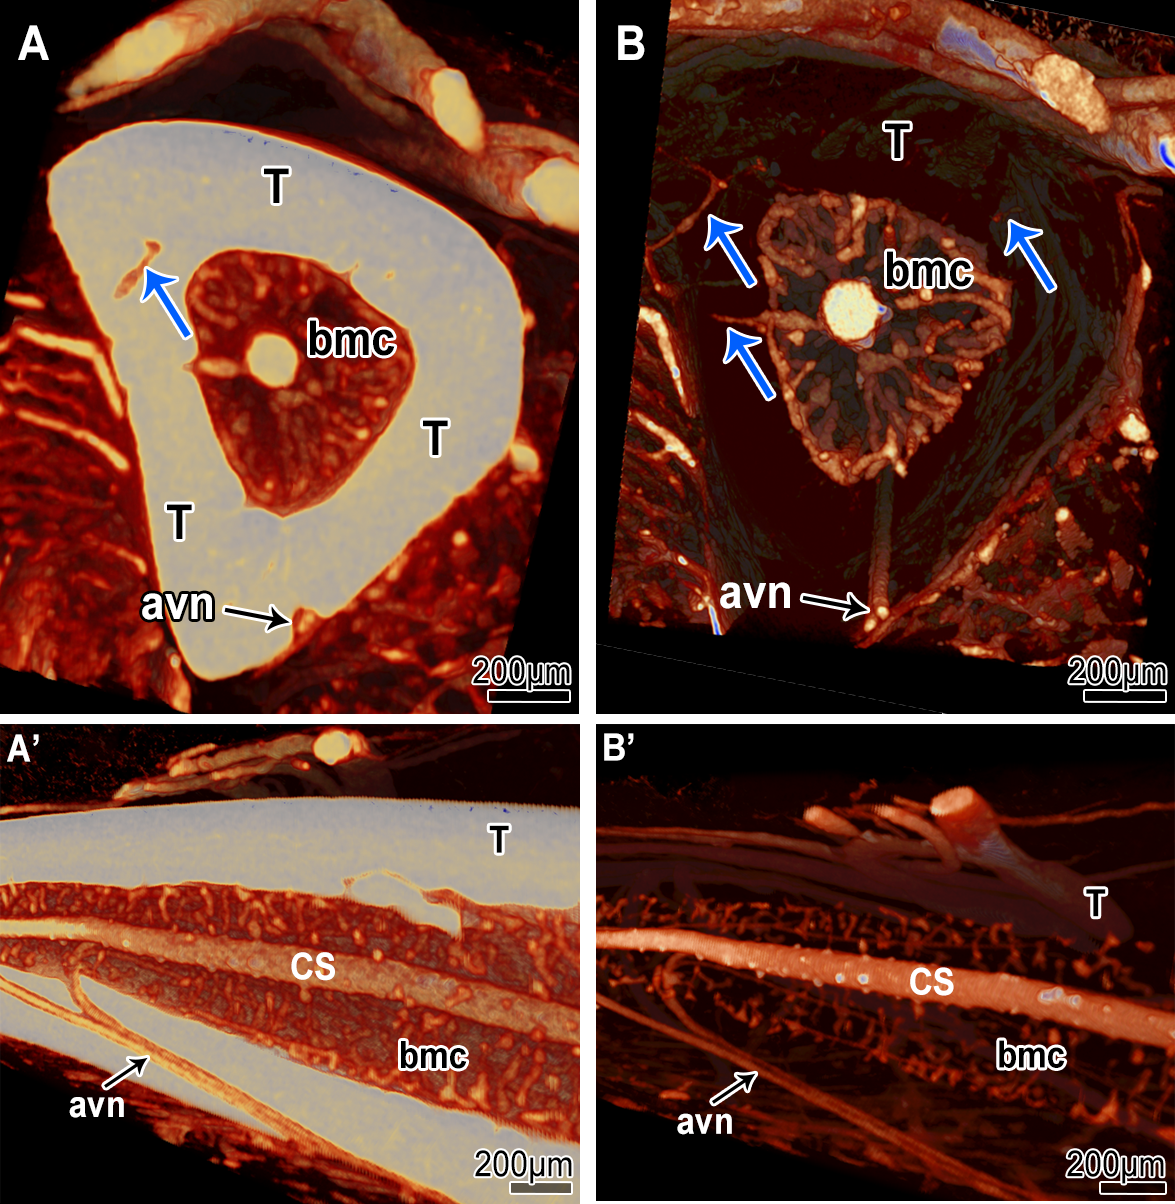
\includegraphics{images/Fig2_Decalcification.png}
\caption{\textbf{microAngioCT-based visualization of the diaphysis of CB17SCID mice tibia before (A \& A') and after decalcification with 10\% EDTA (B \& B').}
In A and A' the tibia bone appears brighter and opaque due to higher X-ray absorption.
In B and B' the tibia bone appears transparent due to its lowered X-ray absorption after decalcification.
Due to the decalcification, connecting vessels between the periosteal vessels and the vessels of the bone marrow cavity (bmc) are more easily detectable (blue arrows in A vs.~B).
The visualization of the vessels within the medullar cavity (\emph{central sinus} (CS)) is also improved.
At the external surface of the tibia, supplying arteries are visible (\emph{arteria et vena nutricia} (avn)).
The structure of the bone tissue is no longer clearly detectable after the decalcification (B-B').}\label{fig:2}
}
\end{figure}

\hypertarget{bone-metastatic-disease-model-microangioct}{%
\paragraph{Bone metastatic disease model, microAngioCT}\label{bone-metastatic-disease-model-microangioct}}

As mentioned in the introduction, simultaneous imaging of bone and vasculature is crucial in a bone metastatic disease model.
Since changes in bone and vasculature are believed to be of crucial importance for the progression of bone metastatic disease, decalcifying the bone tissue is highly unfavorable.

To verify the suitability of our microAngioCT approach for imaging intratumoral vasculature in native, non-decalcified bone tissue we used the following murine bone metastatic disease model.
50000 PC3-M-Pro4Luc2 dTomato cells were injected into the tibia of 6-week-old CB17SCID male mice as previously described\textsuperscript{\protect\hyperlink{ref-C9ratYNO}{39},\protect\hyperlink{ref-16lhxZOpa}{40}}.
The X-ray assessment (25 kV, 6 sec, Faxitron Bioptics, Tucson, Arizona, US) was conducted on days 7, 14, 21, and 28 after implantation to monitor the progression of the lesions.
Before perfusion with μAngiofil (as described above), the hind limb of interest was X-rayed using Faxitron Bioptics as a standard follow-up in this model (see insert in Fig. \ref{fig:3}, Panel A).
The harvested and fixated murine hind limb (4 \% PFA at 4 °C) was then imaged using a desktop microCT scanner (SkyScan 1272, control software 1.1.19, Bruker microCT N.V., Kontich, Belgium) (Fig. \ref{fig:3}) with an X-ray source acceleration voltage of 60 kV and an X-ray source current of 166 μA.
The X-rays were filtered by 0.25 mm of aluminum.
Projection images were recorded over a sample rotation of 180°, with one projection acquired at every 0.1° with 3 projections averaged for noise reduction.
Each projection image with a size of 4904 x 3280 pixels was exposed for 2800 ms.
This resulted in an isotropic voxel size of 1.65 μm.

The visualization (CTvox (v.3.3.1), Bruker microCT N.V., Kontich, Belgium) displays intratumoral vasculature and extensive defects in mineralized bone tissue.
Neighboring structures, such as the growth plate and the epiphysis or the menisci are also easily assessed (Fig. \ref{fig:3}).

\begin{figure}
\hypertarget{fig:3}{%
\centering
\includegraphics{images/Fig3_tumor_tibia.png}
\caption{\textbf{microAngioCT of a xenograft tumor implanted into tibia of 6-week-old CB17SCID male mice.}
A: Maximum intensity projection (MIP) of the three-dimensional dataset of the investigated hind limb segment indicated in the inserted X-ray image of the mouse prior to harvesting.
Inset: X-ray image before sample harvesting.
B: Virtual section through the microAngioCT dataset visualizing remarkable defects represented as holes (asterisks in B and C) in the tibial bone at the tumor site (encircled).
C: A more deeply positioned virtual section displaying the inner surface of the diseased tibia.
Besides irregularly patterned tumor vessels (in B \& C) further bony structures like the growth plate or calcified parts of the medial meniscus (MM) are clearly distinguishable.}\label{fig:3}
}
\end{figure}

\hypertarget{microangioct-of-murine-mandible-and-teeth}{%
\paragraph{microAngioCT of murine mandible and teeth}\label{microangioct-of-murine-mandible-and-teeth}}

C57BL/6 mice were anesthetized (with a mixture of fentanyl (0.05 mg/kg), midazolam (5 mg/kg), and medetomidine (0.5 mg/kg)), and their head was perfused with μAngiofil as described above.
The perfused head was harvested and fixed (4 \% PFA at 4 °C).
Before tomographic imaging the mandible was excised, wrapped in a paper towel, and scanned in a sealed pipette tip.

The mouse teeth were imaged using a desktop microCT scanner (SkyScan 1172 (Version F, control software version 1.5 (build 23)), Bruker microCT N.V., Kontich, Belgium) (Fig. \ref{fig:4}), with an X-ray source acceleration voltage of 80 kV and an X-ray source current of 124 μA.
The X-rays were filtered by 0.5 mm of aluminum.
Projection images were recorded over a sample rotation of 360°, with one projection acquired at every 0.1° with 4 projections averaged for noise reduction.
Each projection image with a size of 4000 x 2672 pixels was exposed for 6260 ms.
This resulted in an isotropic voxel size of 1 μm.

The microvasculature of the murine mandible, periodontal ligament, and the teeth (even within their pulp chamber) can be clearly visualized without undergoing a decalcification procedure (Fig. \ref{fig:4}).

\begin{figure}
\hypertarget{fig:4}{%
\centering
\includegraphics{images/Fig4_mouse_teeth.png}
\caption{\textbf{microAngioCT of the vasculature of C57BL/6 mice teeth.}
A: View onto a virtual section parallel to the crowns of the murine teeth: pulp chambers are visible, and the pulpal vessels are presented.
The inset shows a full view of the tomographic dataset.
B: Sagittal section through the mandible.
The microvessels within the pulp cavities and root canals are distinguishable.
C: Detailed view of the dentogingival plexus and periodontal ligament vessels (PLV).}\label{fig:4}
}
\end{figure}

\hypertarget{microangioct-of-the-mandible-in-a-large-animal-model-guxf6ttingen-minipig}{%
\paragraph{microAngioCT of the mandible in a large animal model (Göttingen Minipig)}\label{microangioct-of-the-mandible-in-a-large-animal-model-guxf6ttingen-minipig}}

Göttingen minipigs (Ellegaard Göttingen Minipig, Dalmose, Denmark) were anesthetized intramuscularly (25--35 mg/kg, Dexdomitor; Orion Pharma Animal Health and 50--70 mg/kg, Zoletil 100 Vet, Virbac) and intravenously heparinized with 300 IE/kg (Heparin LEO, LEO Pharma).
After heparin infusion, the pigs were euthanized with an intravenous dose (100 mg/kg) of pentobarbital (Euthanimal vet, VM Pharma).
The external carotid artery was accessed by blunt dissection through the tissue of the ventral neck and cannulated (BD Venflon, 17G).
After washing out the blood with PBS, the corresponding head side was selectively perfused with μAngiofil through the arterial tree.
Otherwise, the perfusion was performed with the same approach as in the previously described mice experiments.
After the polymerization of μAngiofil, we excised the mandible and fixated and stored it in a 4 \% PFA solution at 4 °C.

Mandibles were then scanned with a SkyScan 1273 (control software version 1.1, Bruker microCT N.V., Kontich, Belgium) (Fig. \ref{fig:5}).
The scans were performed with an X-ray source acceleration voltage of 100 kV and an X-ray source current of 80 μA.
The X-rays were filtered by 1 mm of aluminum and 0.2 mm of copper.
For the visualization shown in panel A, we recorded projection images with a size of 3072 x 1944 pixels over a sample rotation of 360°, with one projection acquired at every 0.1° with 5 projections averaged for noise reduction.
Each projection image was exposed for 225 ms.
This resulted in an isotropic voxel size of 21 μm.
For the visualizations shown in panels B and C, the sample was rotated over 360° with one projection acquired at every 0.15°, and 5 projections averaged for noise reduction.
In addition, two horizontally overlapping projections were stitched to one projection with a size of 4832 x 1944 px to increase the imaged sample volume.
Each projection image was exposed for 225 ms.
This resulted in an isotropic voxel size of 9 μm.

\begin{figure}
\hypertarget{fig:5}{%
\centering
\includegraphics{images/Fig5_Vreni_jaw_minipig.png}
\caption{\textbf{microAngioCT of the minipig mandibula.}
Panel A displays the visualization of a right minipig hemimandible.
The vasculature at the bone surface is visible.
The framed area in A marks the subvolume represented in panel B at higher magnification.
Panel C displays the transverse section marked in panel B: the pulp chamber and root canal with the corresponding vessels are unambiguously visualized.
Due to the voxel size of 8--9 μm, microvessels with a diameter of 40 μm or less cannot be visualized in such large samples.}\label{fig:5}
}
\end{figure}

Osseointegration of implants is influenced by angiogenesis.
As such, studying angiogenesis and, correspondingly the vascular supply of the peri-implant tissue in detail is important for dental research and many implantology studies.
So far, the only reliable approach to assess the vascular supply remains histology, limited to single two-dimensional sections.

While microCT imaging allows for non-destructive, fully 3D imaging of dental research samples with implants, such imaging presents challenges.
This is due to the presence of high-density metal parts with strong X-ray absorption within the samples.
A decalcification step reduces the density of the sample but inevitably leads to the loss of information on the bone microstructure making the simultaneous assessment of the bone and vessels impossible\textsuperscript{\protect\hyperlink{ref-117R9ULnv}{10}}.
To distinguish the vasculature from both the metal implants and the mineralized bone tissue, we instilled the vasculature with a suitable contrast agent (μAngiofil).
The X-ray absorption characteristics of μAngiofil make it possible to visualize and differentiate between soft tissue, bone tissue, contrast agent-filled vessels as well as metal (titanium) implants.
We imaged an μAngiofil-instilled minipig hemimandibula with a SkyScan 2214 (control software version 1.0.0, Bruker microCT N.V., Kontich, Belgium) (Fig. \ref{fig:6}), with an X-ray source acceleration voltage of 100 kV and an X-ray source current of 100 μA.
The X-rays were filtered by 1 mm of copper.
Projection images were recorded over a sample rotation of 360°, with one projection acquired at every 0.18° with 4 projections averaged for noise reduction.
Each projection image with a size of 2929 x 1944 pixels was exposed for 1080 ms.
This resulted in an isotropic voxel size of 8 μm.

In the resulting tomographic datasets these regions of interest can easily be distinguished based on their gray value ranges, as shown in Fig. \ref{fig:6}, Panel C.
Tomographic imaging of such samples and straightforward segmentation of features of interest without cumbersome post-processing (Fig. \ref{fig:6}, Panel D) is enabled without requiring a decalcification step.

\begin{figure}
\hypertarget{fig:6}{%
\centering
\includegraphics{images/Fig6_Segmentation.png}
\caption{\textbf{microAngioCT of the peri-implant vasculature of a minipig mandibula.}
Panel A: Maximum intensity projection image of the minipig mandible dataset with four metal implants and μAngiofil-perfused vessels.
Panel B: virtual transversal section through the dataset showing an implant within the mandible.
The colored circles mark structures with different gray value ranges.
Corresponding peaks with color legend are marked on the histogram in panel C.
Such differences in gray levels allow a straightforward segmentation of the structures of interest as displayed in the 3D visualization in panel D.}\label{fig:6}
}
\end{figure}

Unfortunately, not all samples exhibit a pronounced difference in gray values between bone tissue and μAngiofil when scanned using standard scanning parameters.
This issue is particularly common in murine samples, even though the bone mineral density of mouse bones is generally higher than that of other experimental species\textsuperscript{\protect\hyperlink{ref-FXSWRzX2}{41},\protect\hyperlink{ref-1AEVcopFo}{42}}.
As a result, the gray levels of bone tissue and μAngiofil appear similar, making it impossible to distinguish them based on histogram levels alone (e.g., Fig. \ref{fig:4}).
While decalcification can improve contrast (see Fig. \ref{fig:2}), we propose an alternative, more efficient solution: dual-energy scanning.
Previous studies have demonstrated that microscopic dual-energy CT imaging (microDECT) using commercial lab-based microCT systems can achieve spectral separation of two or more materials with micrometer resolution\textsuperscript{\protect\hyperlink{ref-191glo5Hi}{43},\protect\hyperlink{ref-w1AGMK3j}{44}}.
Notably, the contrasting properties of hydroxyapatite (the primary mineral in bone and teeth) and iodine (the high-Z component in μAngiofil) make them ideal for spectral X-ray imaging\textsuperscript{\protect\hyperlink{ref-191glo5Hi}{43},\protect\hyperlink{ref-ZKU6zNgr}{45},\protect\hyperlink{ref-oRhGUhqB}{46}}.

We evaluated multiple energies (accelerating voltages from 40 to 110 kV) to choose the optimal combination for imaging of the murine mandible perfused with μAngiofil using a SkyScan 2214 (control software version 1.8, Bruker microCT N.V., Kontich, Belgium) (Fig. \ref{fig:7}).
The optimal dual-energy settings for the X-ray source were 50 kV/120 µA and 90 kV/100 µA (acceleration voltage/source current).
Projection images were recorded over a sample rotation of 360°, with one projection acquired at every 0.1° with 7 projections averaged for noise reduction.
Each projection image with a size of 4032 x 2688 pixels was exposed for 6000 ms (on average).
This resulted in datasets with an isotropic voxel size of 1.4 μm.

In comparison to 50 kV, at 90 kV the gray value of the bone tissue was decreased and the gray value of μAngiofil increased (Fig. \ref{fig:7} C').
Such changes allow a non-complicated segmentation of bone and μAngiofil based on the combined histogram (Fig. \ref{fig:7} C'\,').

\begin{figure}
\hypertarget{fig:7}{%
\centering
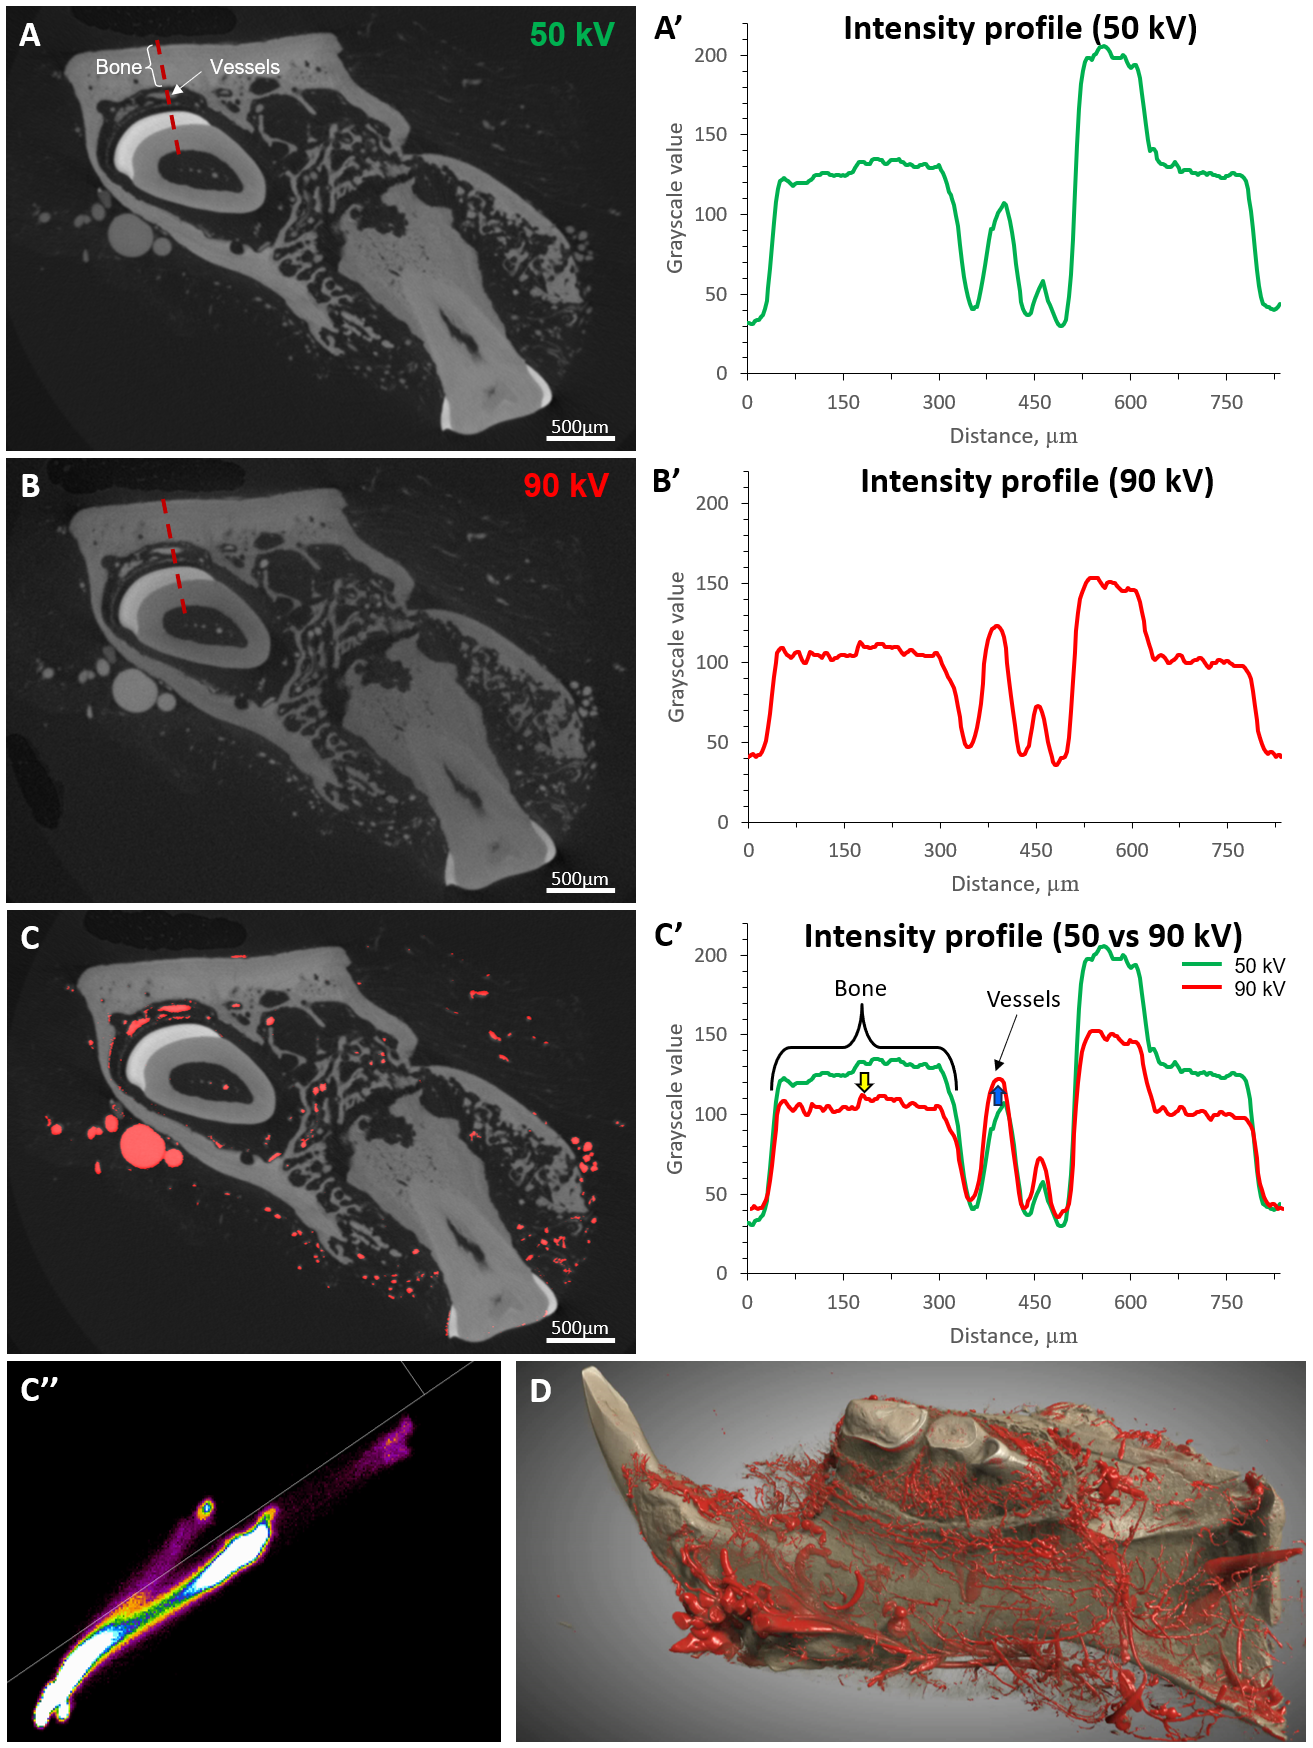
\includegraphics{images/Fig7_DualEnergy.png}
\caption{\textbf{Dual-energy microAngioCT of a murine mandibula.}
Panel A and B represent virtual sections through the microCT datasets obtained at different accelerating voltages: 50 kV (A) and 90 kV (B).
The dashed red line in panels A and B represents the location of the corresponding intensity profile displayed in panels A' and B'.
Panel C represents segmented vasculature using the dual-energy approach.
The changes in the intensity profiles of different tissues are shown in graph C': with the higher voltage (90 kV) the intensity of bone tissue reduces (yellow arrow) and the intensity of vessels (μAngiofil) increases.
Such changes in gray levels allow segmentation of the vessels using the combined histogram shown in panel C'\,' (DEhist, Bruker microCT N.V., Kontich, Belgium).
Panel D represents a three-dimensional visualization of the segmented tissues (Dragonfly 3D World (2024.1), Comet Technologies Canada Inc., Montréal, Canada).}\label{fig:7}
}
\end{figure}

\hypertarget{discussion}{%
\subsection{Discussion}\label{discussion}}

Adequate vascularization is a prerequisite for successful bone formation and regeneration as well as osseointegration of biomaterials\textsuperscript{\protect\hyperlink{ref-zXoIXG3G}{1},\protect\hyperlink{ref-lVl4gVyN}{47}--\protect\hyperlink{ref-16mB4VUpP}{50}}.
Without high-resolution imaging, the interplay between vasculature and bone tissue cannot be adequately studied, making it impossible to control these processes.

Non-destructive microCT imaging is is widely regarded as the only viable method for 3D imaging of an intact bone-implant interface\textsuperscript{\protect\hyperlink{ref-11349lK8v}{26}}.
To accurately differentiate vasculature from other soft tissue structures, the use of a contrast agent or the creation of a vascular replica is essential.

The imaging method we present, which involves instillation with μAngiofil, addresses several limitations of previously described techniques (see \protect\hyperlink{introduction}{Introduction}).
This approach enables the visualization of both bone tissue and the microvasculature within it, with or without prior decalcification (Fig. \ref{fig:2}).''**

The established decalcifying protocols enable correlative imaging of the same sample with preserved intravascular contrast agent with subsequent classical histological evaluation\textsuperscript{\protect\hyperlink{ref-iM9i6gkJ}{38}}.
Such a decalcification step enables tomographic imaging of the murine hind limb vasculature with fewer artifacts around the bone at lower acceleration voltages of the X-ray source due to the reduced radiopacity of the sample.
Such lower acceleration voltages often enable shortened scanning times, leading to a higher sample throughput.
Furthermore, decalcifying the sample enables a threshold-based segmentation of the vasculature, and facilitates histological evaluation of the sample, as previously described\textsuperscript{\protect\hyperlink{ref-iM9i6gkJ}{38}}.
However, the decalcification step renders bone tissue transparent, disabling simultaneous 3D imaging of the bony and vascular structures.

In many models, due to the distinct differences in the X-ray attenuation of μAngiofil and the bone tissue, we can forgo the time-consuming decalcification step.
This permits us direct assessment of vascularization and bone growth in a single scan (Fig. \ref{fig:6}).
While effective, this approach does not always yield optimal results (e.g., Fig. \ref{fig:4}).
Although decalcification is a viable option for quite some studies, a dual-energy scanning technique offers a more efficient solution (Fig. \ref{fig:7}).
By conducting two sequential scans without removing the sample, this method simplifies dataset registration, avoids the time-consuming decalcification step, and provides simultaneous imaging of bone and vasculature while keeping the sample intact.
Therefore, the microAngioCT approach we present here can be used for the simultaneous visualization of hard and soft tissues and their vascularization in small and large animal models.

One of the noteworthy possible applications of this approach is the simultaneous visualization of the bone microarchitecture and microvasculature of bone metastases in a murine xenograft tumor model (Fig. \ref{fig:3}).
Especially for studying bone metastatic models, it is crucial to find a method that allows for the correct assessment of the microvasculature without decalcifying the sample.
Such a decalcification would hinder the thorough assessment of pathological processes in bone tissue.
These pathological processes can cause skeletal-related events, which are associated with shortened survival and deterioration of quality of life\textsuperscript{\protect\hyperlink{ref-D7D7Wyla}{51}}, and should therefore be avoided.
Our method allows studying the response to specific treatments, including bone-targeted and antiangiogenic therapies.
These can be assessed in 3D within the same sample, and be followed up with a histological examination if desired\textsuperscript{\protect\hyperlink{ref-15Cb0RCtH}{52}}.
The presented method could offer additional insights into the interplay between angiogenesis and bone growth, bone lysis, and bone turnover, which have not been fully elucidated yet.
The potential findings can be crucial for selecting potential drug candidates, proper treatment decisions, and efficacy prediction.

In dental research, preclinical models can be divided into small and large animals.
Small animal models, particularly mice and rats, are highly popular, due to their practical size and cost-effectiveness.
The microCT scan of correspondingly small samples, perfused with μAngiofil can be performed with a voxel size of around 1 μm, providing excellent detail resolution (Fig. \ref{fig:4}).
Murine mandibles and teeth are challenging for assessing the vasculature.
This is due to the location of most of the vessels within the bone canals or in the proximity of the hard tissue.
This consequently leads to the lack of larger bone-free volumes in which the vasculature is easily distinguishable.
Gray value-based segmentation of bone and contrast-agent-instilled vasculature is compounded by the fact that murine bone has a higher mineral bone density when compared to other species\textsuperscript{\protect\hyperlink{ref-FXSWRzX2}{41},\protect\hyperlink{ref-1AEVcopFo}{42}}.
Nonetheless, with the dual-energy approach described above, we achieved appropriate imaging of such samples and were able to visualize and distinguish vasculature in/from mineralized bone tissue.

In the small animal model studies without metal or similar biomedical implants, the application of whole mouse clearing and imaging with vDISCO approach could be the method of choice\textsuperscript{\protect\hyperlink{ref-BNZSaEBe}{14}}.
Another promising improvement to the clearing protocols and immunolabeling of the samples with the bone tissue is the introduction of the collagenase digestion step, which improves the antibody penetration throughout the stained bones and, therefore, the immunostaining\textsuperscript{\protect\hyperlink{ref-ZGzobRpX}{11}}.
Although newer tissue clearing and immunostaining immersion-based visualization techniques provide high-resolution, three-dimensional images of intact samples, these methods may produce artifacts such as tissue deformation and illumination inhomogeneity\textsuperscript{\protect\hyperlink{ref-yP3RkDdM}{18}}.

The presence of implanted biomedical devices further complicates the imaging process.
For murine model studies, a recently published tissue-clearing-based imaging approach\textsuperscript{\protect\hyperlink{ref-11349lK8v}{26}} could be a viable option for the visualization of the peri-implant tissues and vasculature due to the small size of hemimandible samples and the availability of transgenic mouse lines.
However, there are limitations to such a tissue-clearing imaging approach.
Namely:
i) differential shrinkage among soft and hard tissues, leading to anisotropic distortion in samples where both tissue types (plus eventual metal implant) are present;
ii) limited imaging depth (approximately 800 μm in a mouse model\textsuperscript{\protect\hyperlink{ref-11349lK8v}{26}}) due to the challenges of achieving complete transparency of bone tissue.
Significant anisotropic distortion of the sample may alter the implant-tissue interface, a common site of interest.
The limitation of the maximal achievable imaging depth makes such an approach impractical for usage in large animal models.

Our presented microAngioCT approach does not have such limitations and can be easily applied for visualization of hemimandible and its vascularization in a large animal model like Göttingen minipig (Fig. \ref{fig:5}).
μAngiofil exhibits significantly different attenuation properties than mineralized bone in most species and allows for distinction, segmentation and visualization of soft tissue, bone tissue, vessels filled with the contrast agent as well as metal implants according to their gray values in the histogram (Fig. \ref{fig:6}).

To the best of our knowledge, our study is the first to demonstrate non-destructive 3D imaging of the microvasculature of bone in the proximity of metal objects/implants in a large animal model.

\hypertarget{limitations-of-our-approach}{%
\subsubsection{Limitations of our approach}\label{limitations-of-our-approach}}

Achieving the excellent results demonstrated in this study requires reproducible and controlled instillation of the contrast agent.
To ensure this, the procedure should be performed by skilled personnel using a syringe pump.
While other contrast agents may be somewhat easier to use for instillation, they do not deliver the same high-quality results, as previously discussed.

The method we presented for investigating the microvasculature within bone tissue is primarily limited by the imaging technique.
Specifically, this limitation arises from the correlation between achievable resolution and the physical size of the imaged sample.
For small samples, such as those just a few millimeters in diameter, voxel sizes on the order of 1 μm enable visualization of the microvasculature down to the capillary bed\textsuperscript{\protect\hyperlink{ref-s9aC9H1e}{35}--\protect\hyperlink{ref-iM9i6gkJ}{38}}.
However, for larger samples, such as the minipig hemimandible, the achievable voxel size is approximately 10 times larger (≥8 μm).
In such cases, the finest microvessels with diameters under 40 μm cannot be accurately visualized (see Fig. \ref{fig:5} \& \ref{fig:6}).

Beyond the inherent limitations of tomographic imaging, the approach presented here---instilling the vasculature in bone tissue with a polymerizing contrast agent---marks a significant advancement in both qualitative and quantitative imaging.
This innovative method holds great promise for addressing key questions in tissue engineering, implantology, and a wide range of related research fields.''

\hypertarget{author-contributions}{%
\subsection{Author Contributions}\label{author-contributions}}

\href{https://credit.niso.org/}{Contributor Roles Taxonomy}, as defined by the \href{https://credit.niso.org/contributor-roles-defined/}{National Information Standards Organization}.

\begin{tablenos:no-prefix-table-caption}

\begin{longtable}[]{@{}
  >{\raggedright\arraybackslash}p{(\columnwidth - 2\tabcolsep) * \real{0.5000}}
  >{\raggedright\arraybackslash}p{(\columnwidth - 2\tabcolsep) * \real{0.5000}}@{}}
\toprule()
\begin{minipage}[b]{\linewidth}\raggedright
Author
\end{minipage} & \begin{minipage}[b]{\linewidth}\raggedright
Contributions
\end{minipage} \\
\midrule()
\endhead
David Haberthür & Data curation; Formal analysis; Investigation; Project administration; Software; Validation; Visualization; Writing -- original draft; Writing -- review \& editing \\
Oleksiy-Zakhar Khoma & Data curation; Formal analysis; Investigation; Project administration; Software; Validation; Visualization; Writing -- original draft; Writing -- review \& editing \\
Tim Hoessly & Data curation; Investigation; Writing -- review \& editing \\
Eugenio Zoni & Investigation; Methodology; Resources; Writing -- review \& editing \\
Marianna Kruithof-de Julio & Methodology; Resources; Writing -- review \& editing \\
Stewart D. Ryan & Resources; Writing -- review \& editing \\
Myriam Grunewald & Investigation; Methodology; Resources; Writing -- review \& editing \\
Benjamin Bellón & Investigation; Methodology; Writing -- review \& editing \\
Rebecca Sandgren & Investigation; Writing -- review \& editing \\
Stephan Handschuh & Methodology; Writing -- review \& editing \\
Benjamin E. Pippenger & Funding acquisition; Investigation; Methodology; Resources; Writing -- review \& editing \\
Dieter Bosshardt & Methodology; Writing -- review \& editing \\
Valentin Djonov & Conceptualization; Funding acquisition; Resources; Writing -- review \& editing \\
Ruslan Hlushchuk & Conceptualization; Funding acquisition; Investigation; Methodology; Project administration; Resources; Supervision; Validation; Visualization; Writing -- original draft; Writing -- review \& editing \\
\bottomrule()
\end{longtable}

\end{tablenos:no-prefix-table-caption}

\hypertarget{conflicts-of-interest}{%
\subsection{Conflicts of interest}\label{conflicts-of-interest}}

\begin{tablenos:no-prefix-table-caption}

\begin{longtable}[]{@{}ll@{}}
\toprule()
Author & Conflict \\
\midrule()
\endhead
Benjamin Bellón & Employed by a company producing dental implants \\
Benjamin E. Pippenger & Employed by a company producing dental implants \\
\bottomrule()
\end{longtable}

\end{tablenos:no-prefix-table-caption}

\hypertarget{acknowledgments}{%
\subsection{Acknowledgments}\label{acknowledgments}}

We are grateful to the \href{https//www.mic.unibe.ch/}{Microscopy Imaging Center} of the University of Bern for infrastructural support.
We thank the \texttt{manubot} project\textsuperscript{\protect\hyperlink{ref-YuJbg3zO}{53}} for helping us write this manuscript collaboratively.

\hypertarget{supplementary-materials}{%
\subsection{Supplementary Materials}\label{supplementary-materials}}

\hypertarget{log-files-of-all-the-tomographic-scans-performed-for-this-study}{%
\subsubsection{Log files of all the tomographic scans performed for this study}\label{log-files-of-all-the-tomographic-scans-performed-for-this-study}}

The CSV file \href{https://github.com/microct-ana-unibe-ch/microvasculature-manuscript/blob/main/content/data/ScanningDetails.csv}{ScanningDetails.csv} gives a tabular overview of all the (relevant) parameters of all the scans we performed.
This file was generated with a \href{https://github.com/habi/BrukerSkyScanLogfileRuminator}{data processing notebook} and contains information read from \emph{all} the log files of \emph{all} the scans we performed.
A copy of each log file is available \href{https://github.com/microct-ana-unibe-ch/microvasculature-manuscript/tree/main/content/data}{online}.

\hypertarget{data-availability}{%
\subsection{Data availability}\label{data-availability}}

Each of the tomographic datasets used and analyzed during the current study is available from the corresponding author upon reasonable request.

\hypertarget{references}{%
\subsection{References}\label{references}}

\hypertarget{refs}{}
\begin{CSLReferences}{0}{0}
\leavevmode\vadjust pre{\hypertarget{ref-zXoIXG3G}{}}%
\CSLLeftMargin{1. }%
\CSLRightInline{Wernike, E. \emph{et al.} \href{https://doi.org/10.1002/jbm.a.32411}{Long‐term cell‐mediated protein release from calcium phosphate ceramics}. \emph{J Biomedical Materials Res} \textbf{92A}, 463--474 (2009).}

\leavevmode\vadjust pre{\hypertarget{ref-AHsHFIUt}{}}%
\CSLLeftMargin{2. }%
\CSLRightInline{Roche, B. \emph{et al.} \href{https://doi.org/10.1016/j.bone.2011.09.051}{Structure and quantification of microvascularisation within mouse long bones: What and how should we measure?} \emph{Bone} \textbf{50}, 390--399 (2012).}

\leavevmode\vadjust pre{\hypertarget{ref-1FaKEBtU8}{}}%
\CSLLeftMargin{3. }%
\CSLRightInline{Carulli, C., Innocenti, M. \& Brandi, M. L. \href{https://doi.org/10.3389/fendo.2013.00106}{Bone Vascularization in Normal and Disease Conditions}. \emph{Front. Endocrinol.} \textbf{4}, (2013).}

\leavevmode\vadjust pre{\hypertarget{ref-yZTJBX1B}{}}%
\CSLLeftMargin{4. }%
\CSLRightInline{Filipowska, J., Tomaszewski, K. A., Niedźwiedzki, Ł., Walocha, J. A. \& Niedźwiedzki, T. \href{https://doi.org/10.1007/s10456-017-9541-1}{The role of vasculature in bone development, regeneration and proper systemic functioning}. \emph{Angiogenesis} \textbf{20}, 291--302 (2017).}

\leavevmode\vadjust pre{\hypertarget{ref-Vu36g0cK}{}}%
\CSLLeftMargin{5. }%
\CSLRightInline{Ren, Y., Senarathna, J., Grayson, W. L. \& Pathak, A. P. \href{https://doi.org/10.1152/ajpcell.00195.2022}{State-of-the-art techniques for imaging the vascular microenvironment in craniofacial bone tissue engineering applications}. \emph{American Journal of Physiology-Cell Physiology} \textbf{323}, C1524--C1538 (2022).}

\leavevmode\vadjust pre{\hypertarget{ref-dBkW39I8}{}}%
\CSLLeftMargin{6. }%
\CSLRightInline{Kuttappan, S. \emph{et al.} \href{https://doi.org/10.1016/j.actbio.2018.07.050}{Dual release of growth factor from nanocomposite fibrous scaffold promotes vascularisation and bone regeneration in rat critical sized calvarial defect}. \emph{Acta Biomaterialia} \textbf{78}, 36--47 (2018).}

\leavevmode\vadjust pre{\hypertarget{ref-Es64ZQO}{}}%
\CSLLeftMargin{7. }%
\CSLRightInline{Kurobane, T. \emph{et al.} \href{https://doi.org/10.1016/j.actbio.2019.02.021}{Angiogenesis involvement by octacalcium phosphate-gelatin composite-driven bone regeneration in rat calvaria critical-sized defect}. \emph{Acta Biomaterialia} \textbf{88}, 514--526 (2019).}

\leavevmode\vadjust pre{\hypertarget{ref-5mgeUNd6}{}}%
\CSLLeftMargin{8. }%
\CSLRightInline{Grosso, A. \emph{et al.} \href{https://doi.org/10.3389/fbioe.2017.00068}{It Takes Two to Tango: Coupling of Angiogenesis and Osteogenesis for Bone Regeneration}. \emph{Front. Bioeng. Biotechnol.} \textbf{5}, (2017).}

\leavevmode\vadjust pre{\hypertarget{ref-33Vq8bQx}{}}%
\CSLLeftMargin{9. }%
\CSLRightInline{Lovett, M., Lee, K., Edwards, A. \& Kaplan, D. L. \href{https://doi.org/10.1089/ten.teb.2009.0085}{Vascularization Strategies for Tissue Engineering}. \emph{Tissue Engineering Part B: Reviews} \textbf{15}, 353--370 (2009).}

\leavevmode\vadjust pre{\hypertarget{ref-117R9ULnv}{}}%
\CSLLeftMargin{10. }%
\CSLRightInline{Núñez, J. A. \emph{et al.} \href{https://doi.org/10.1038/s41598-017-13632-5}{Simultaneous visualisation of calcified bone microstructure and intracortical vasculature using synchrotron X-ray phase contrast-enhanced tomography}. \emph{Sci Rep} \textbf{7}, (2017).}

\leavevmode\vadjust pre{\hypertarget{ref-ZGzobRpX}{}}%
\CSLLeftMargin{11. }%
\CSLRightInline{Biswas, L. \emph{et al.} \href{https://doi.org/10.1016/j.cell.2022.12.031}{Lymphatic vessels in bone support regeneration after injury}. \emph{Cell} \textbf{186}, 382--397.e24 (2023).}

\leavevmode\vadjust pre{\hypertarget{ref-DiX3YTwQ}{}}%
\CSLLeftMargin{12. }%
\CSLRightInline{Rindone, A. N. \emph{et al.} \href{https://doi.org/10.1038/s41467-021-26455-w}{Quantitative 3D imaging of the cranial microvascular environment at single-cell resolution}. \emph{Nat Commun} \textbf{12}, (2021).}

\leavevmode\vadjust pre{\hypertarget{ref-X0aG1K2m}{}}%
\CSLLeftMargin{13. }%
\CSLRightInline{Luo, W. \emph{et al.} \href{https://doi.org/10.1089/scd.2019.0104}{Investigation of Postnatal Craniofacial Bone Development with Tissue Clearing-Based Three-Dimensional Imaging}. \emph{Stem Cells and Development} \textbf{28}, 1310--1321 (2019).}

\leavevmode\vadjust pre{\hypertarget{ref-BNZSaEBe}{}}%
\CSLLeftMargin{14. }%
\CSLRightInline{Cai, R. \emph{et al.} \href{https://doi.org/10.1038/s41596-022-00788-2}{Whole-mouse clearing and imaging at the cellular level with vDISCO}. \emph{Nat Protoc} \textbf{18}, 1197--1242 (2023).}

\leavevmode\vadjust pre{\hypertarget{ref-1FUMXJVtA}{}}%
\CSLLeftMargin{15. }%
\CSLRightInline{Mercado-Pagán, Á. E., Stahl, A. M., Shanjani, Y. \& Yang, Y. \href{https://doi.org/10.1007/s10439-015-1253-3}{Vascularization in Bone Tissue Engineering Constructs}. \emph{Ann Biomed Eng} \textbf{43}, 718--729 (2015).}

\leavevmode\vadjust pre{\hypertarget{ref-KjvwGWK2}{}}%
\CSLLeftMargin{16. }%
\CSLRightInline{Harrison, K. D. \& Cooper, D. M. L. \href{https://doi.org/10.3389/fendo.2015.00122}{Modalities for Visualization of Cortical Bone Remodeling: The Past, Present, and Future}. \emph{Front. Endocrinol.} \textbf{6}, (2015).}

\leavevmode\vadjust pre{\hypertarget{ref-168Ee16HU}{}}%
\CSLLeftMargin{17. }%
\CSLRightInline{Schneider, P. \emph{et al.} \href{https://doi.org/10.1002/jemt.20720}{Simultaneous 3D visualization and quantification of murine bone and bone vasculature using micro‐computed tomography and vascular replica}. \emph{Microscopy Res \&amp; Technique} \textbf{72}, 690--701 (2009).}

\leavevmode\vadjust pre{\hypertarget{ref-yP3RkDdM}{}}%
\CSLLeftMargin{18. }%
\CSLRightInline{Rosenblum, J. S. \emph{et al.} \href{https://doi.org/10.1016/j.crmeth.2021.100151}{Non-invasive in situ visualization of the murine cranial vasculature}. \emph{Cell Reports Methods} \textbf{2}, 100151 (2022).}

\leavevmode\vadjust pre{\hypertarget{ref-13YRlKdu2}{}}%
\CSLLeftMargin{19. }%
\CSLRightInline{Young, S. \emph{et al.} \href{https://doi.org/10.1089/ten.teb.2008.0153}{Microcomputed Tomography Characterization of Neovascularization in Bone Tissue Engineering Applications}. \emph{Tissue Engineering Part B: Reviews} \textbf{14}, 295--306 (2008).}

\leavevmode\vadjust pre{\hypertarget{ref-DWiXWNoA}{}}%
\CSLLeftMargin{20. }%
\CSLRightInline{Krucker, T., Lang, A. \& Meyer, E. P. \href{https://doi.org/10.1002/jemt.20263}{New polyurethane‐based material for vascular corrosion casting with improved physical and imaging characteristics}. \emph{Microscopy Res \&amp; Technique} \textbf{69}, 138--147 (2006).}

\leavevmode\vadjust pre{\hypertarget{ref-KJUjdwi7}{}}%
\CSLLeftMargin{21. }%
\CSLRightInline{Perrien, D. S. \emph{et al.} \href{https://doi.org/10.1186/s12882-016-0235-5}{Novel methods for microCT-based analyses of vasculature in the renal cortex reveal a loss of perfusable arterioles and glomeruli in eNOS-/- mice}. \emph{BMC Nephrol} \textbf{17}, (2016).}

\leavevmode\vadjust pre{\hypertarget{ref-Ror9Uhfa}{}}%
\CSLLeftMargin{22. }%
\CSLRightInline{Leyssens, L., Pestiaux, C. \& Kerckhofs, G. \href{https://doi.org/10.3390/ijms22063263}{A Review of Ex Vivo X-ray Microfocus Computed Tomography-Based Characterization of the Cardiovascular System}. \emph{IJMS} \textbf{22}, 3263 (2021).}

\leavevmode\vadjust pre{\hypertarget{ref-1A0HsmRho}{}}%
\CSLLeftMargin{23. }%
\CSLRightInline{Hong, S. \emph{et al.} \href{https://doi.org/10.1002/jnr.24539}{Development of barium‐based low viscosity contrast agents for micro CT vascular casting: Application to 3D visualization of the adult mouse cerebrovasculature}. \emph{J of Neuroscience Research} \textbf{98}, 312--324 (2019).}

\leavevmode\vadjust pre{\hypertarget{ref-cNoYNu8B}{}}%
\CSLLeftMargin{24. }%
\CSLRightInline{Hlushchuk, R., Barré, S. \& Djonov, V. Morphological Aspects of Tumor Angiogenesis. in \emph{Methods in Molecular Biology} 13--24 (Springer New York, 2016). doi:\href{https://doi.org/10.1007/978-1-4939-3999-2_2}{10.1007/978-1-4939-3999-2\_2}.}

\leavevmode\vadjust pre{\hypertarget{ref-18wESlA6d}{}}%
\CSLLeftMargin{25. }%
\CSLRightInline{Jing, X. L. \emph{et al.} \href{https://doi.org/10.1055/s-0032-1329540}{Radiomorphometric Quantitative Analysis of Vasculature Utilizing Micro--Computed Tomography and Vessel Perfusion in the Murine Mandible}. \emph{Craniomaxillofacial Trauma \&amp; Reconstruction} \textbf{5}, 223--229 (2012).}

\leavevmode\vadjust pre{\hypertarget{ref-11349lK8v}{}}%
\CSLLeftMargin{26. }%
\CSLRightInline{Yi, Y. \emph{et al.} \href{https://doi.org/10.1111/cpr.12578}{3‐dimensional visualization of implant‐tissue interface with the polyethylene glycol associated solvent system tissue clearing method}. \emph{Cell Proliferation} \textbf{52}, (2019).}

\leavevmode\vadjust pre{\hypertarget{ref-rCXuqa0O}{}}%
\CSLLeftMargin{27. }%
\CSLRightInline{Raphel, J., Holodniy, M., Goodman, S. B. \& Heilshorn, S. C. \href{https://doi.org/10.1016/j.biomaterials.2016.01.016}{Multifunctional coatings to simultaneously promote osseointegration and prevent infection of orthopaedic implants}. \emph{Biomaterials} \textbf{84}, 301--314 (2016).}

\leavevmode\vadjust pre{\hypertarget{ref-X5Wzek9s}{}}%
\CSLLeftMargin{28. }%
\CSLRightInline{Hsieh, J. \emph{Computed Tomography: Principles, Design, Artifacts, and Recent Advances}. (SPIE Optical Engineering Press, Bellingham, WA, 2003).}

\leavevmode\vadjust pre{\hypertarget{ref-137VU0bph}{}}%
\CSLLeftMargin{29. }%
\CSLRightInline{Bai, L. \emph{et al.} \href{https://doi.org/10.1016/j.actbio.2018.06.023}{Differential effect of hydroxyapatite nano-particle versus nano-rod decorated titanium micro-surface on osseointegration}. \emph{Acta Biomaterialia} \textbf{76}, 344--358 (2018).}

\leavevmode\vadjust pre{\hypertarget{ref-Siy9vGW7}{}}%
\CSLLeftMargin{30. }%
\CSLRightInline{Wang, S., Liu, Y., Fang, D. \& Shi, S. \href{https://doi.org/10.1111/j.1601-0825.2006.01337.x}{The miniature pig: a useful large animal model for dental and orofacial research}. \emph{Oral Diseases} \textbf{13}, 530--537 (2007).}

\leavevmode\vadjust pre{\hypertarget{ref-i45b7Cmp}{}}%
\CSLLeftMargin{31. }%
\CSLRightInline{\emph{et al.} \href{https://doi.org/10.22203/ecm.v013a01}{Animal models for implant biomaterial research in bone: A review}. \emph{eCM} \textbf{13}, 1--10 (2007).}

\leavevmode\vadjust pre{\hypertarget{ref-1EXdAADA3}{}}%
\CSLLeftMargin{32. }%
\CSLRightInline{Bellinger, D., Merricks, E. \& Nichols, T. Minipig Models of Diabetes Mellitus. in \emph{The Minipig in Biomedical Research} 445--468 (CRC Press, 2011). doi:\href{https://doi.org/10.1201/b11356-37}{10.1201/b11356-37}.}

\leavevmode\vadjust pre{\hypertarget{ref-nC0ZZVgL}{}}%
\CSLLeftMargin{33. }%
\CSLRightInline{Grunewald, M. \emph{et al.} \href{https://doi.org/10.1126/science.abc8479}{Counteracting age-related VEGF signaling insufficiency promotes healthy aging and extends life span}. \emph{Science} \textbf{373}, (2021).}

\leavevmode\vadjust pre{\hypertarget{ref-1ppOkyPO}{}}%
\CSLLeftMargin{34. }%
\CSLRightInline{Percie du Sert, N. \emph{et al.} \href{https://doi.org/10.1371/journal.pbio.3000411}{Reporting animal research: Explanation and elaboration for the ARRIVE guidelines 2.0}. \emph{PLoS Biol} \textbf{18}, e3000411 (2020).}

\leavevmode\vadjust pre{\hypertarget{ref-s9aC9H1e}{}}%
\CSLLeftMargin{35. }%
\CSLRightInline{Hlushchuk, R. \emph{et al.} \href{https://doi.org/10.1007/s00429-020-02158-8}{Innovative high-resolution microCT imaging of animal brain vasculature}. \emph{Brain Struct Funct} \textbf{225}, 2885--2895 (2020).}

\leavevmode\vadjust pre{\hypertarget{ref-ijqzbOI6}{}}%
\CSLLeftMargin{36. }%
\CSLRightInline{Hlushchuk, R. \emph{et al.} \href{https://doi.org/10.1152/ajprenal.00099.2017}{Cutting-edge microangio-CT: new dimensions in vascular imaging and kidney morphometry}. \emph{American Journal of Physiology-Renal Physiology} \textbf{314}, F493--F499 (2018).}

\leavevmode\vadjust pre{\hypertarget{ref-TYAmre95}{}}%
\CSLLeftMargin{37. }%
\CSLRightInline{Hlushchuk, R., Haberthür, D. \& Djonov, V. \href{https://doi.org/10.1016/j.vph.2018.09.003}{Ex vivo microangioCT: Advances in microvascular imaging}. \emph{Vascular Pharmacology} \textbf{112}, 2--7 (2019).}

\leavevmode\vadjust pre{\hypertarget{ref-iM9i6gkJ}{}}%
\CSLLeftMargin{38. }%
\CSLRightInline{Schaad, L. \emph{et al.} \href{https://doi.org/10.1038/srep41842}{Correlative Imaging of the Murine Hind Limb Vasculature and Muscle Tissue by MicroCT and Light Microscopy}. \emph{Sci Rep} \textbf{7}, (2017).}

\leavevmode\vadjust pre{\hypertarget{ref-C9ratYNO}{}}%
\CSLLeftMargin{39. }%
\CSLRightInline{Zoni, E. \emph{et al.} \href{https://doi.org/10.1158/1541-7786.mcr-18-1220}{Therapeutic Targeting of CD146/MCAM Reduces Bone Metastasis in Prostate Cancer}. \emph{Molecular Cancer Research} \textbf{17}, 1049--1062 (2019).}

\leavevmode\vadjust pre{\hypertarget{ref-16lhxZOpa}{}}%
\CSLLeftMargin{40. }%
\CSLRightInline{Dai, J., Hensel, J., Wang, N., Kruithof-de Julio, M. \& Shiozawa, Y. \href{https://doi.org/10.1038/bonekey.2016.4}{Mouse models for studying prostate cancer bone metastasis}. \emph{BoneKEy Reports} \textbf{5}, (2016).}

\leavevmode\vadjust pre{\hypertarget{ref-FXSWRzX2}{}}%
\CSLLeftMargin{41. }%
\CSLRightInline{Entezari, V. \emph{et al.} \href{https://doi.org/10.1016/j.bone.2011.10.004}{Further improvements on the factors affecting bone mineral density measured by quantitative micro-computed tomography}. \emph{Bone} \textbf{50}, 611--618 (2012).}

\leavevmode\vadjust pre{\hypertarget{ref-1AEVcopFo}{}}%
\CSLLeftMargin{42. }%
\CSLRightInline{INUI, A. \emph{et al.} \href{https://doi.org/10.1292/jvms.66.599}{Age-Related Changes of Bone Mineral Density and Microarchitecture in Miniature Pigs}. \emph{J. Vet. Med. Sci.} \textbf{66}, 599--609 (2004).}

\leavevmode\vadjust pre{\hypertarget{ref-191glo5Hi}{}}%
\CSLLeftMargin{43. }%
\CSLRightInline{HANDSCHUH, S., BEISSER, C. J., RUTHENSTEINER, B. \& METSCHER, B. D. \href{https://doi.org/10.1111/jmi.12543}{Microscopic dual‐energy CT (microDECT): a flexible tool for multichannel\textless i\textgreater ex vivo\textless/i\textgreater3D imaging of biological specimens}. \emph{Journal of Microscopy} \textbf{267}, 3--26 (2017).}

\leavevmode\vadjust pre{\hypertarget{ref-w1AGMK3j}{}}%
\CSLLeftMargin{44. }%
\CSLRightInline{Handschuh, S., Reichart, U., Kummer, S. \& Glösmann, M. In situ isotropic 3D imaging of vasculature perfusion specimens using x‐ray microscopic dual‐energy CT. \emph{Journal of Microscopy} (2024) doi:\href{https://doi.org/10.1111/jmi.13369}{10.1111/jmi.13369}.}

\leavevmode\vadjust pre{\hypertarget{ref-ZKU6zNgr}{}}%
\CSLLeftMargin{45. }%
\CSLRightInline{Fornaro, J. \emph{et al.} \href{https://doi.org/10.1007/s13244-010-0057-0}{Dual- and multi-energy CT: approach to functional imaging}. \emph{Insights Imaging} \textbf{2}, 149--159 (2011).}

\leavevmode\vadjust pre{\hypertarget{ref-oRhGUhqB}{}}%
\CSLLeftMargin{46. }%
\CSLRightInline{Kruger, R. A., Riederer, S. J. \& Mistretta, C. A. \href{https://doi.org/10.1118/1.594374}{Relative properties of tomography, \textless i\textgreater K\textless/i\textgreater‐edge imaging, and \textless i\textgreater K\textless/i\textgreater‐edge tomography}. \emph{Medical Physics} \textbf{4}, 244--249 (1977).}

\leavevmode\vadjust pre{\hypertarget{ref-lVl4gVyN}{}}%
\CSLLeftMargin{47. }%
\CSLRightInline{Li, Y. \emph{et al.} \href{https://doi.org/10.1021/acsabm.1c00979}{Tissue Engineered Neurovascularization Strategies for Craniofacial Tissue Regeneration}. \emph{ACS Appl. Bio Mater.} \textbf{5}, 20--39 (2021).}

\leavevmode\vadjust pre{\hypertarget{ref-Ha1wHU4s}{}}%
\CSLLeftMargin{48. }%
\CSLRightInline{Schott, N. G., Friend, N. E. \& Stegemann, J. P. \href{https://doi.org/10.1089/ten.teb.2020.0132}{Coupling Osteogenesis and Vasculogenesis in Engineered Orthopedic Tissues}. \emph{Tissue Engineering Part B: Reviews} \textbf{27}, 199--214 (2021).}

\leavevmode\vadjust pre{\hypertarget{ref-zB5E7Obz}{}}%
\CSLLeftMargin{49. }%
\CSLRightInline{Sivaraj, K. K. \& Adams, R. H. \href{https://doi.org/10.1242/dev.136861}{Blood vessel formation and function in bone}. \emph{Development} \textbf{143}, 2706--2715 (2016).}

\leavevmode\vadjust pre{\hypertarget{ref-16mB4VUpP}{}}%
\CSLLeftMargin{50. }%
\CSLRightInline{Chandra, P. \& Atala, A. \href{https://doi.org/10.1042/cs20180155}{Engineering blood vessels and vascularized tissues: technology trends and potential clinical applications}. \emph{Clinical Science} \textbf{133}, 1115--1135 (2019).}

\leavevmode\vadjust pre{\hypertarget{ref-D7D7Wyla}{}}%
\CSLLeftMargin{51. }%
\CSLRightInline{D\textquotesingle Oronzo, S., Coleman, R., Brown, J. \& Silvestris, F. \href{https://doi.org/10.1016/j.jbo.2018.10.004}{Metastatic bone disease: Pathogenesis and therapeutic options}. \emph{Journal of Bone Oncology} \textbf{15}, 100205 (2019).}

\leavevmode\vadjust pre{\hypertarget{ref-15Cb0RCtH}{}}%
\CSLLeftMargin{52. }%
\CSLRightInline{Xu, H. \emph{et al.} \href{https://doi.org/10.3390/cancers14143443}{Impact of Anti-Angiogenic Treatment on Bone Vascularization in a Murine Model of Breast Cancer Bone Metastasis Using Synchrotron Radiation Micro-CT}. \emph{Cancers} \textbf{14}, 3443 (2022).}

\leavevmode\vadjust pre{\hypertarget{ref-YuJbg3zO}{}}%
\CSLLeftMargin{53. }%
\CSLRightInline{Himmelstein, D. S. \emph{et al.} \href{https://doi.org/10.1371/journal.pcbi.1007128}{Open collaborative writing with Manubot}. \emph{PLoS Comput Biol} \textbf{15}, e1007128 (2019).}

\end{CSLReferences}
